\chapter{Methodology and experiment}

\section{Survey}
The survey is a part of this thesis. The survey is used to answer different hypothesis around geospatial micro tasks. To be able to answer the hypothesises three tasks containing the same two questions was developed. The questions will represent two different micro-tasks, while the three tasks will contain one, three and six elements that the participant will use to answer the questions with. The participant will always answers the two question's on six elements, but the tasks vary how many element's need's to be handled at the same time. The variation of number of elements in the task's is to hopefully find out if the number of elements in an micro-task effects how well people solves the task. 

There are two variable types used in this survey, dependent- and independent variables. The dependent variables are time, number of correctly chosen elements in both questions and also difficulty. The independent variables are number of elements in the task, experienced or non-experienced participant, gender, age and if the participant know micro tasking.

\section{Web-application}
This thesis used an online web-based survey to conduct the experiment. An online survey avoid the cost and effort of printing, distributing, and collecting paper forms. Many people prefer to answer a brief survey displayed on a screen instead of filling in and returning a printed form \citep{Ben2009}.   

In a self selected sample, which is some the case here, there is potentially a bias in the sample \citep{Ben2009}. %s168

\section{Pilot test}
It is important to pilot test the survey prior to actual use \citep{Ben2009}. A pilot test provides an opportunity to validate the wording of the tasks, do the participants understand the tasks? It also helps understand the time necessary for completing the survey, which should be communicated to the participants in prior to the survey \citep{Schade2015}. The pilot-test will be conducted with a small sample of users. Results from the pilot test kan be used to do improvements to the actual survey, to the web-application hosting the survey and to find errors or weaknesses in the databasemodels.

After the pilot test the usability was measured. The standard ISO 9241-11 suggests that measures of usability should cover effectiveness, efficiency and satisfaction \citep{ISO1998}. Measuring these three classes of metric can vary widely and makes it difficult to make comparisons of usability between different systems. "[...] just because a particular design feature has proved to be very useful in making one system usable does not necessarily mean that it will do so for another system" \citep{Brooke1996}. Usability in this thesis will be measured with the \textit{System Usability Scale}(SUS) because it gives an subjective measure of usability. The \textit{System Usability Scale} questionnaire consists of ten statements where the participants rate their agreement in an five-point scale \citep{Ben2009}. Subjective measure of usability is usually obtained through the use of questionnaire and attitude scales \citep{Brooke1996}. SUS was developed to be quick and simple, but also reliable enough to be able to compare performance changes between versions \citep{Brooke1996}. It is also easy to administer the participants through the usability test and it can be used on small sample sizes an still give reliable results \citep{Affairs2013}.  

The usability is important to measure. If the participants doesn't understand how the web-application works, they will probably not do the survey since they then have to invest time in understanding what to do. %they will either exit the survey or answer the questions in the survey wrong. 
It is also important to get enough participants to do the whole survey and not quit halfway in frustration of not understanding it properly. The \textit{System Usability Scale} can effectively differantiate between usable and unusable systems \citep{Affairs2013}. 

\subsection{Execution of the pilot test}
The pilot test was conducted with a total of eight participants, five experienced and three non-experienced participants aged from 22 to 64 years. It started with a brief information about this study and the survey. They where told to talk out load during the survey, no help or guidance was given to the participants. The author observed the participants while they conducted the survey. The author took notes and watched if the participants understood the questions in the survey correctly. After the survey a \textit{System Usability Scale} questionnaire was answered by the participants. At the end the participants was asked to give general feedback on the web-application. The SUS score and the feedback was then used to determine the usability of the web-application and to determine which improvements to be done.  

\subsection{Results from the pilot test}

- Did someone knew micro-tasking? Can we see something here?

The average SUS score was 84.64 out of 100. Anything above 68 is considered above average \citep{Affairs2013}. When adding the SUS score to an adjective rating will an score of 85.5 or higher be described as excellent \citep{Bangor2009}. A score of 84.64 is then described as good/excellent. 

All participants thought that the instruction movie was confusing. It was short, the instructions went too fast and it lacked voice descriptions. The movie needed major improvements, an important discovery. The purpose of the movie is to give the participant an introduction to how to answer the two questions. It gives important instructions, especially for participants that are not used to working with maps on a web page. 

Overall feedback on question one was that it was difficult to understand which building was which and also when a building layer was selected or not. The lack of labels on the buildings was done on purpose to get the task as much as possible realistic. The prosess of selecting the best building layer needed improvements, it had to be clearer that selection was done by clicking on the layer on the map, not by using the layer control as some thought. This was added to the movie with voice description. The design on the question one page was also improved by adding color to the text telling the participant which layer was selected. 
 
Some pages also had too much information and long sentences. The task progress bar was removed, no one noticed it, only the survey progress bar on the top right is necessary. 

The two oldest participants spent almost twice as much time on the test than the younger. Maybe it where too much cognitive load on them. Learning a new application and at the same time understanding how to do the survey and answer the questions given to them. One of them where experienced and the other non-experienced, so this is a surprising result.  CHECK THE TIME ON EACH TASK FOR THE OLDER PARTICIPANTS. Figure \ref{fig:allparticipantssortedageparticipantexclude4labelage} show the task results from all participants ordered by age. There are three entries per participant, so three and three bars are results from the same participant. \newline

\begin{figure}[h]
	\centering
	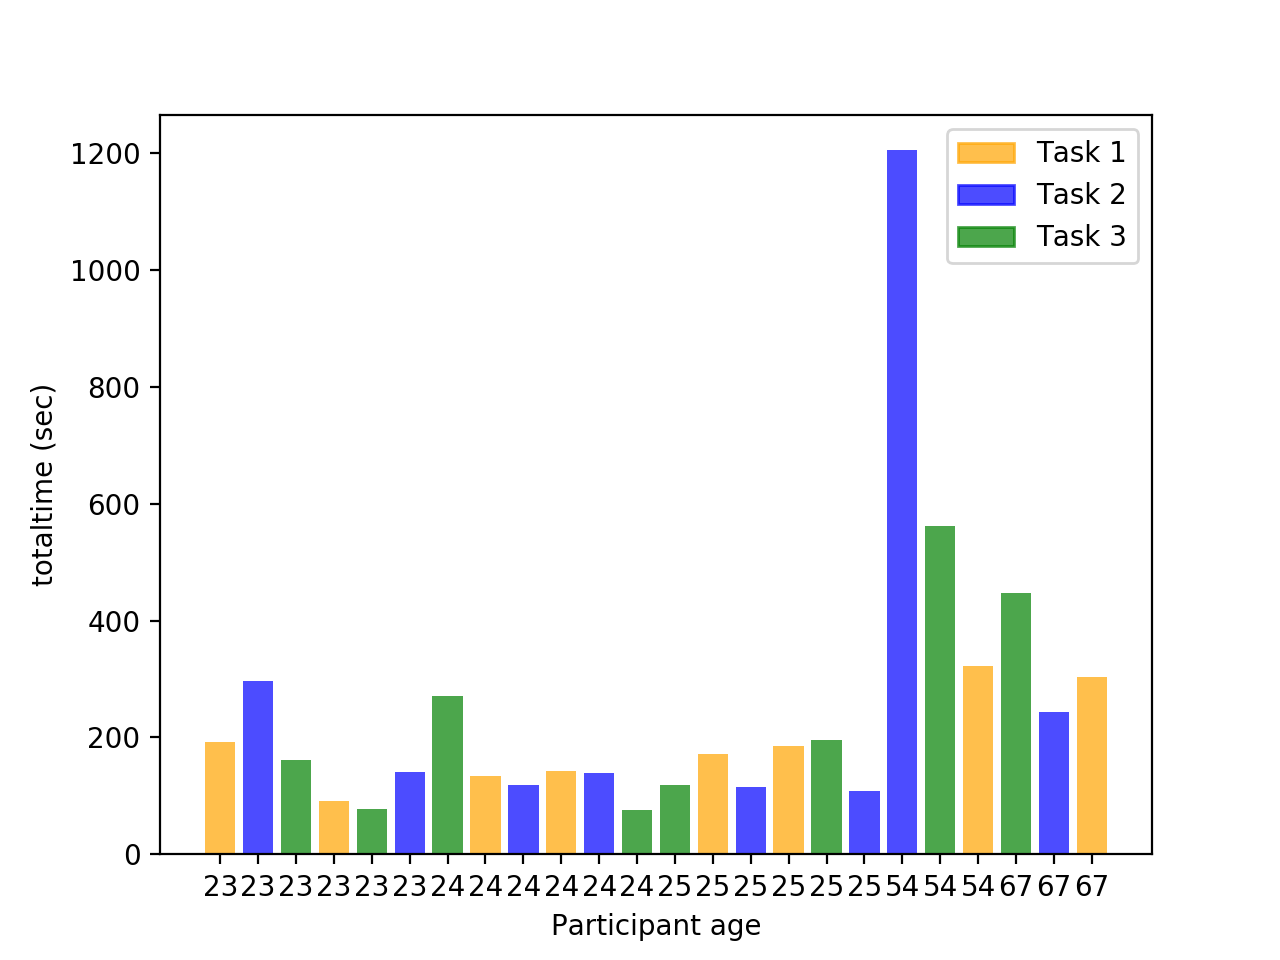
\includegraphics[width=0.8\linewidth]{fig/allParticipants_sorted_Age_Participant_exclude4_labelage}
	\caption[totaltimeage]{Total time - all participants ordered by age}
	\label{fig:allparticipantssortedageparticipantexclude4labelage}
\end{figure}

The average time spent on the survey was 18 minutes. The two oldest participants used on average 33 minutes, while the rest of the participants spent on average 13 minutes to complete the survey. 

The pilot test data was used to test some of the hypothesis to find errors or weaknesses in the databasemodel. The data was extracted with the help of Django QuerySets and saved in csv files. There were a few errors and weaknesses found, most of them are listed under: 

\begin{enumerate}
	\item Add foreign key from TaskResult model to TaskSurvey
	\item Added four other fields in TaskResult model
	\begin{itemize}
		\item Total correct elements 
		\item Task order
		\item Task number
		\item List of correctly chosen building numbers in both questions
	\end{itemize}
\end{enumerate}

The additional fields will maninly help with creating plots to better interpret the data and to more easily visualize the different results. 

%\subsubsection{Statistics result}
%First the pilot-test result need to be normality tested. 
%As mentioned in \ref{subsec:normaltesting} this thesis will use the Anderson-Darling test. The python library Scipy has an Anderson-Darling test function \citep{TheScipycommunity2017}, this was used to answer the normality test with the Anderson-Darling hypothesis. Testing the total time data form all participants (in total 32 entries) in Anderson-Darling gave a \textit{p-value} of 0.717. The null hypothesis cannot be rejected, then there are two possible cases. One can either accept the null hypothesis or the sample size is not large enough to either accept or reject the null hypothesis \citep{ThePennsylvaniaStateUniversity2017}. An acceptance of the null hypothesis implies that the evidence was insufficient, the result does not necessary accept $H_{0}$, but fails to reject $H_{0}$ \citep{Walpole2012}.  

\begin{framed}{\noindent\centering
\textit{Anderson-Darling test} \\
\textbf{Data:} All participants - total time, 32 entries\\
  \textbf{P-value:} 0.717  \\
    \textit{P-value} > 0.05\\
  \textbf{$H_{0}$:} Accepted, failed to reject
  \par}
\end{framed}


\section[Sample Size]{Determining the sample size}
The sample size is influenced by a number of factors, including the purpose of the study, population size, the risk of selecting a "bad" sample and the allowable sampling error \citep{Israel1992}. In this survey there are three possible ways of determining the sample size. 

\begin{figure}[h]
	\centering
	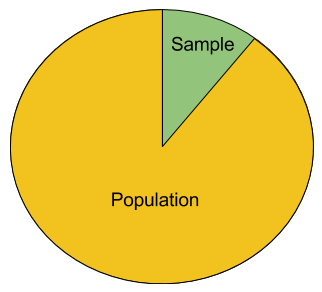
\includegraphics[width=0.35\linewidth]{fig/popsample}
	\caption{Population vs. sample}
	\label{fig:popsample}
\end{figure}

A sample is a collection of observations and is the subset of a population, illustrated in figure \ref{fig:popsample}. The population size in this survey is not easily determined. A population is the collection of individuals of a particular type \citep{Walpole2012}. All individuals with access to a computer and internet interested in contributing to micro-tasks is basicly the population. 

There are three possible ways of determining the sample size in this study. The first option is to use a sample size from a similair study. The risk is to repeat errors that were made in determining the sample for another study. The second option is to rely on published tables, depending on precision, confidence levels, and variability. According to \cite{Israel1992} table 1, a precision of 0.05, confidence level of 95\% and a size of population greater than 100'000, the neccessary sample size is 400. If the precision is changed to 0.1, the sample size neccessary increases to 100 \citep{Israel1992}. The numbers found in the table reflects the number of obtained responses. The last approach is to use formulas to calculate the sample size. The formulas requires the standard deviation and how much variance to expect in the response \citep{Smith2013}\citep{Israel1992}. \cite{Israel1992} mentions that the table gives a useful guide for determening the sample size, and that formulas are used if the study has a different combination of precision and confidence. This study will use the table result since the combinations matches this study.

It's important to mention that the quality of the sample is as important as it's size. The more variable the sampled data is, the larger the sample size is required \citep{Israel1992}. It's also desirable to choose a random sample, which means that the observations are made idependently and random. The main purpose of using a random sample is to obtain correct information about the unknown population parameters \citep{Walpole2012}. 

%Results from the pilot-test can be used to determine the sample size. The sample size tells us how many responses that are needed to make inferences about a population as a whole \citep{Smith2013}. The formula for determining the sample size requires the standard deviation, how much variance to expect in the response \citep{Smith2013}. This standard deviation can be calculated from the pilot test results. Determining sample size is a very important issue because samples that are too large may waste time, resources and money, while samples that are too small may lead to inaccurate result. Equation \ref{eq:samplesize} show how to calculate the sample size, n. 

%\begin{equation}\label{eq:samplesize}
%n = [\frac{z_{\frac{\alpha}{2}}^2 \sigma (1-\sigma)}{e^2}]
%\end{equation}

%Using the results from all participants, excluding the training task, and using data from the column total time, the standardeviation is 184.8 and mean value 156.1 seconds.  
